\documentclass[11pt]{article}
\usepackage[margin=2.5cm]{geometry}
\usepackage{booktabs}
\usepackage{graphicx}
\usepackage{placeins}
\usepackage{natbib}
\usepackage{hyperref}
\usepackage{setspace}
\usepackage{helvet}
\renewcommand{\familydefault}{\sfdefault}

\setstretch{1.15}

\title{Bullying and Reading Achievement: A Comparison of South Africa and Brazil Using PIRLS 2021}
\author{Chane Watt \\ Stellenbosch University}
\date{\today}

\begin{document}
\maketitle

\section{Abstract}
What is the association between bullying exposure and reading achievement among Grade 4 students in South Africa, and how does this association compare with Brazil?
Possible hypotheses:
- Students experiencing more frequent bullying have lower reading achievement.
- The association remains after accounting for demographic and socioeconomic differences.
- The strength of the association may differ by gender or socioeconomic background.
- The association may differ between South Africa and Brazil.

\section{Introduction}

The most prominent headline within the South African education sphere is that 81\% of grade 4 learners can not read for meaning. Many studies have attempted to find the underlying mechanisms that resulted in these low test scores with the natural inclination coming to mind being learners social economic status, the school quantile or the confidence of the learners. In 2016 however \citet{anton_erxleben2016bullying} found that bullying is one of the key drivers of lower  academic performance illustrated in their Directed Acyclic Graph results. 

\section{Literature Review}
Find roughly 10–15 strong studies on bullying and educational achievement.
Prioritise PIRLS/TIMSS studies, South African evidence, and comparable middle-income countries.
Record each paper’s bullying measure, outcome, controls, method, and main result.
Use this to construct a simple conceptual framework and select covariates

•	bullying and academic achievement;
•	bullying and reading achievement specifically;
•	PIRLS or TIMSS bullying studies;
•	South African bullying research;
•	Brazilian or comparable middle-income-country evidence;
•	gender or socioeconomic differences in bullying effects.
Create a literature matrix with:
Study	Country/data	Bullying measure	Outcome	Controls	Method	Main result	Limitation
The literature review should answer:
1.	Why might bullying affect reading achievement?
2.	Which variables might confound the relationship?
3.	Is there evidence that the relationship differs by gender or SES?
4.	Which variables might be consequences of bullying rather than confounders?
That last question is important. Variables such as absenteeism, school belonging, fear, or engagement may be mechanisms through which bullying affects achievement. Automatically controlling for them could remove part of the relationship you are trying to estimate.


França ()

\section{Data and Methodology}

We use the PIRLS 2021 public-use data for South Africa and Brazil. Rather than importing the R data files manually and reconstructing the complex survey design, we import the official SPSS files using the R package \texttt{EdSurvey}. This package is specifically designed for large-scale education assessments such as PIRLS and automatically recognises the study's sampling weights, jackknife replicate weights, plausible values, and relationships between student and school records.

\subsection{Why EdSurvey Was Selected}

PIRLS does not use a simple random sample. Schools are sampled first, after which classes and students are sampled within schools. Consequently, students have unequal probabilities of selection, while students attending the same school are not statistically independent.

\texttt{EdSurvey} retains the survey-design information required to account for:

\begin{itemize}
    \item the student sampling weight, \texttt{TOTWGT};
    \item stratification and clustering in the PIRLS sample;
    \item the 196 jackknife replicates for Brazil;
    \item the 250 jackknife replicates for South Africa; and
    \item uncertainty associated with the five reading plausible values.
\end{itemize}

Accounting for these features prevents the use of ordinary standard errors, which would generally be underestimated because they do not reflect the complex PIRLS sampling design.

\subsection{Data Loading}

The two countries are imported in R as follows:

\begin{verbatim}
pirls <- readPIRLS(
  path = "data/raw",
  countries = c("zaf", "bra")
)
\end{verbatim}

This produces separate \texttt{EdSurvey} data objects for South Africa and Brazil. The package processes the official PIRLS files and performs the required student--school linking when variables are requested.

\subsection{Variables Prepared}

The \texttt{getData()} function is used to inspect and prepare the variables presented in Table~\ref{tab:pirls_variables}.

\begin{table}[htbp]
    \centering
    \caption{PIRLS variables used in the analysis}
    \label{tab:pirls_variables}
    \begin{tabular}{ll}
        \toprule
        \textbf{Concept} & \textbf{PIRLS variable(s)} \\
        \midrule
        Student identifier      & \texttt{IDSTUD} \\
        School identifier       & \texttt{IDSCHOOL} \\
        Class identifier        & \texttt{IDCLASS} \\
        Gender                  & \texttt{ASBG01} \\
        Home-resources scale    & \texttt{ASBGHRL} \\
        Home-resources category & \texttt{ASDGHRL} \\
        Bullying scale          & \texttt{ASBGSB} \\
        Bullying category       & \texttt{ASDGSB} \\
        Reading achievement     & \texttt{ASRREA01}--\texttt{ASRREA05} \\
        \bottomrule
    \end{tabular}
\end{table}

The variable \texttt{ASBGSB} is a Rasch-scaled measure for which higher values represent less frequent bullying. The categorical variable \texttt{ASDGSB} groups students into ``About Weekly,'' ``About Monthly,'' and ``Almost Never'' categories.

\subsection{Use of Reading Plausible Values}

PIRLS administers only part of the complete reading assessment to each student. Reading achievement is therefore treated as a latent quantity rather than as a conventional observed test score.

PIRLS supplies five plausible values:

\begin{center}
\texttt{ASRREA01}, \texttt{ASRREA02}, \texttt{ASRREA03},
\texttt{ASRREA04}, and \texttt{ASRREA05}.
\end{center}

The regression analysis must be estimated across all five plausible values. The resulting estimates are then combined so that their standard errors incorporate:

\begin{enumerate}
    \item sampling uncertainty arising from observing a sample of students; and
    \item imputation uncertainty arising from the estimation of latent reading achievement.
\end{enumerate}

Using only \texttt{ASRREA01} would ignore part of the imputation uncertainty and would therefore understate the uncertainty surrounding the estimates.

\subsection{Validation Results}

The revised data audit produced the sample counts shown in Table~\ref{tab:sample_counts}.

\begin{table}[htbp]
    \centering
    \caption{Validated PIRLS sample sizes}
    \label{tab:sample_counts}
    \begin{tabular}{lrr}
        \toprule
        \textbf{Country} & \textbf{Students} & \textbf{Schools} \\
        \midrule
        South Africa & 12,422 & 321 \\
        Brazil       & 4,941  & 187 \\
        \bottomrule
    \end{tabular}
\end{table}

Every student identifier is unique, and \texttt{EdSurvey} returns all five reading plausible values for both countries.

\subsection{Treatment of Missing Data}

For the initial data audit, omitted PIRLS response categories are retained so that the full sample can be validated. This prevents the sample from being reduced silently when information on gender, bullying, or home resources is missing.

Missing observations will subsequently be excluded explicitly for each regression specification. This approach makes changes in the analytical sample size transparent.

\subsection{Distinction Between Data Extraction and Estimation}

The \texttt{getData()} function produces an ordinary R data frame that is suitable for checking variables, recoding, and descriptive inspection. It should not be used as a replacement survey design for final statistical inference.

Final weighted tables and regressions will therefore be estimated using the original \texttt{EdSurvey} objects and functions such as \texttt{edsurveyTable()} and \texttt{lm.sdf()}. This preserves the PIRLS sampling weights, plausible-value calculations, and jackknife standard errors.


\section{Results}

Table~\ref{tab:bullying-main-models} presents the M1–M5 estimates for South Africa and Brazil. There is a negative relationship for both Brazil and South Africa between reading scores and bullying penalties. South Africa in Model 1 that just controls for Bullying Penalty indicates a decrease of 55.1 points in reading scores if the learner is bullied on a monthly basis and a decrease of 116.6 points if bullied on a weekly basis. Brazil displays the same negative pattern: learners bullied monthly score 36.4 points lower, while those bullied weekly score 123.5 points lower. All four M1 bullying coefficients are statistically significant at the 1\% level.

The model develops in interesting directions as controls are added in M2, M3, M4 and M5. In South Africa, the estimated bullying penalties become progressively smaller as controls are added, with the M5 coefficients indicating a 36.1-point decrease for monthly bullying and an 80.6-point decrease for weekly bullying. Brazil, by contrast, remains comparatively stable: the monthly penalty increases in magnitude from 36.4 points in M1 to 38.4 points in M5, while the weekly penalty decreases from 123.5 to 113.3 points. The standard errors generally decrease as controls are introduced, indicating greater precision. The explained variance increases from 13.4\% to 38.0\% in South Africa and from 13.9\% to 35.5\% in Brazil.

\begin{table}[!htbp]
\centering
\caption{Bullying and reading achievement: main model sequence}
\label{tab:bullying-main-models}
\scriptsize
\setlength{\tabcolsep}{2.2pt}
\resizebox{\textwidth}{!}{%
\begin{tabular}{lcccccccccc}
\toprule
 & \multicolumn{5}{c}{South Africa} & \multicolumn{5}{c}{Brazil} \\
\cmidrule(lr){2-6}\cmidrule(lr){7-11}
 & M1 & M2 & M3 & M4 & M5 & M1 & M2 & M3 & M4 & M5 \\
\midrule
Bullied about monthly & \shortstack{-55.1***\\(6.9)} & \shortstack{-53.8***\\(6.8)} & \shortstack{-46.8***\\(5.9)} & \shortstack{-43.9***\\(5.5)} & \shortstack{-36.1***\\(5.5)} & \shortstack{-36.4***\\(5.7)} & \shortstack{-37.5***\\(5.4)} & \shortstack{-39.3***\\(5.5)} & \shortstack{-36.5***\\(5.3)} & \shortstack{-38.4***\\(5.8)} \\
Bullied about weekly & \shortstack{-116.5***\\(7.8)} & \shortstack{-110.4***\\(7.5)} & \shortstack{-97.9***\\(6.8)} & \shortstack{-94.2***\\(6.7)} & \shortstack{-80.6***\\(6.7)} & \shortstack{-123.5***\\(7.6)} & \shortstack{-119.2***\\(8.0)} & \shortstack{-112.9***\\(7.3)} & \shortstack{-109.4***\\(7.2)} & \shortstack{-113.3***\\(7.9)} \\
Boy &  & \shortstack{-44.4***\\(3.1)} & \shortstack{-43.4***\\(3.5)} & \shortstack{-40.8***\\(3.8)} & \shortstack{-43.1***\\(3.9)} &  & \shortstack{-10.2**\\(5.0)} & \shortstack{-5.4\\(4.6)} & \shortstack{-3.9\\(4.5)} & \shortstack{-4.9\\(4.8)} \\
Age (years) &  & \shortstack{-10.0***\\(3.0)} & \shortstack{-7.6**\\(3.4)} & \shortstack{-6.9**\\(3.4)} & \shortstack{-7.6**\\(3.3)} &  & \shortstack{-24.6***\\(3.9)} & \shortstack{-13.1***\\(4.4)} & \shortstack{-12.6***\\(4.6)} & \shortstack{-12.7**\\(4.8)} \\
Home SES (ASBHSES scale points) &  &  & \shortstack{25.7***\\(2.3)} & \shortstack{24.9***\\(2.4)} & \shortstack{16.8***\\(2.5)} &  &  & \shortstack{26.3***\\(2.0)} & \shortstack{25.7***\\(2.0)} & \shortstack{21.6***\\(1.8)} \\
Home language: almost always test language &  &  &  & \shortstack{7.4\\(8.1)} & \shortstack{-5.5\\(8.1)} &  &  &  & \shortstack{-18.7*\\(10.7)} & \shortstack{-20.8*\\(10.7)} \\
Home language: sometimes test language &  &  &  & \shortstack{46.3***\\(7.4)} & \shortstack{22.4***\\(7.1)} &  &  &  & \shortstack{7.6\\(9.8)} & \shortstack{12.3\\(9.5)} \\
Home language: never test language &  &  &  & \shortstack{-28.0***\\(8.9)} & \shortstack{-40.7***\\(10.6)} &  &  &  & \shortstack{-93.2***\\(19.2)} & \shortstack{-83.3***\\(19.4)} \\
School location: suburban &  &  &  &  & \shortstack{-18.0\\(17.6)} &  &  &  &  & \shortstack{-1.3\\(15.8)} \\
School location: medium city/large town &  &  &  &  & \shortstack{1.9\\(34.0)} &  &  &  &  & \shortstack{-18.6**\\(9.1)} \\
School location: small town/village &  &  &  &  & \shortstack{-45.1**\\(18.8)} &  &  &  &  & \shortstack{-25.3**\\(11.5)} \\
School location: remote rural &  &  &  &  & \shortstack{-55.5***\\(16.5)} &  &  &  &  & \shortstack{-14.4\\(25.3)} \\
Economically disadvantaged: 11 to 25\% &  &  &  &  & \shortstack{-49.4*\\(27.8)} &  &  &  &  & \shortstack{-25.5**\\(10.9)} \\
Economically disadvantaged: 26 to 50\% &  &  &  &  & \shortstack{-82.8***\\(20.2)} &  &  &  &  & \shortstack{-47.6***\\(13.7)} \\
Economically disadvantaged: more than 50\% &  &  &  &  & \shortstack{-117.3***\\(17.1)} &  &  &  &  & \shortstack{-40.9***\\(11.7)} \\
Other gender category &  &  &  &  &  &  & \shortstack{-100.2***\\(31.1)} & \shortstack{-86.7**\\(35.1)} & \shortstack{-85.6**\\(35.6)} & \shortstack{-49.1**\\(23.6)} \\
\midrule
Learners & 11,660 & 11,618 & 9,167 & 8,505 & 7,177 & 4,715 & 4,706 & 4,110 & 4,022 & 3,563 \\
$R^{2}$ & 0.134 & 0.170 & 0.278 & 0.296 & 0.380 & 0.139 & 0.165 & 0.317 & 0.324 & 0.355 \\
\bottomrule
\end{tabular}%
}
\parbox{0.98\textwidth}{\footnotesize \textit{Notes:} Entries are coefficients with jackknife standard errors in parentheses. The reference group is almost never bullied; the gender reference is girls. All models use the default PIRLS student weight and all five reading plausible values. M1 includes bullying; M2 adds gender and age; M3 adds continuous home SES; M4 adds home language; M5 adds school location and economically disadvantaged composition. Significance: *** p\textless{}0.01, ** p\textless{}0.05, * p\textless{}0.10.}
\end{table}

\FloatBarrier

Figure~\ref{fig:bullying-coefficients} summarizes the bullying coefficients across M1–M5, showing how the estimated associations change as successive controls are introduced.
\begin{figure}[!htbp]
\centering
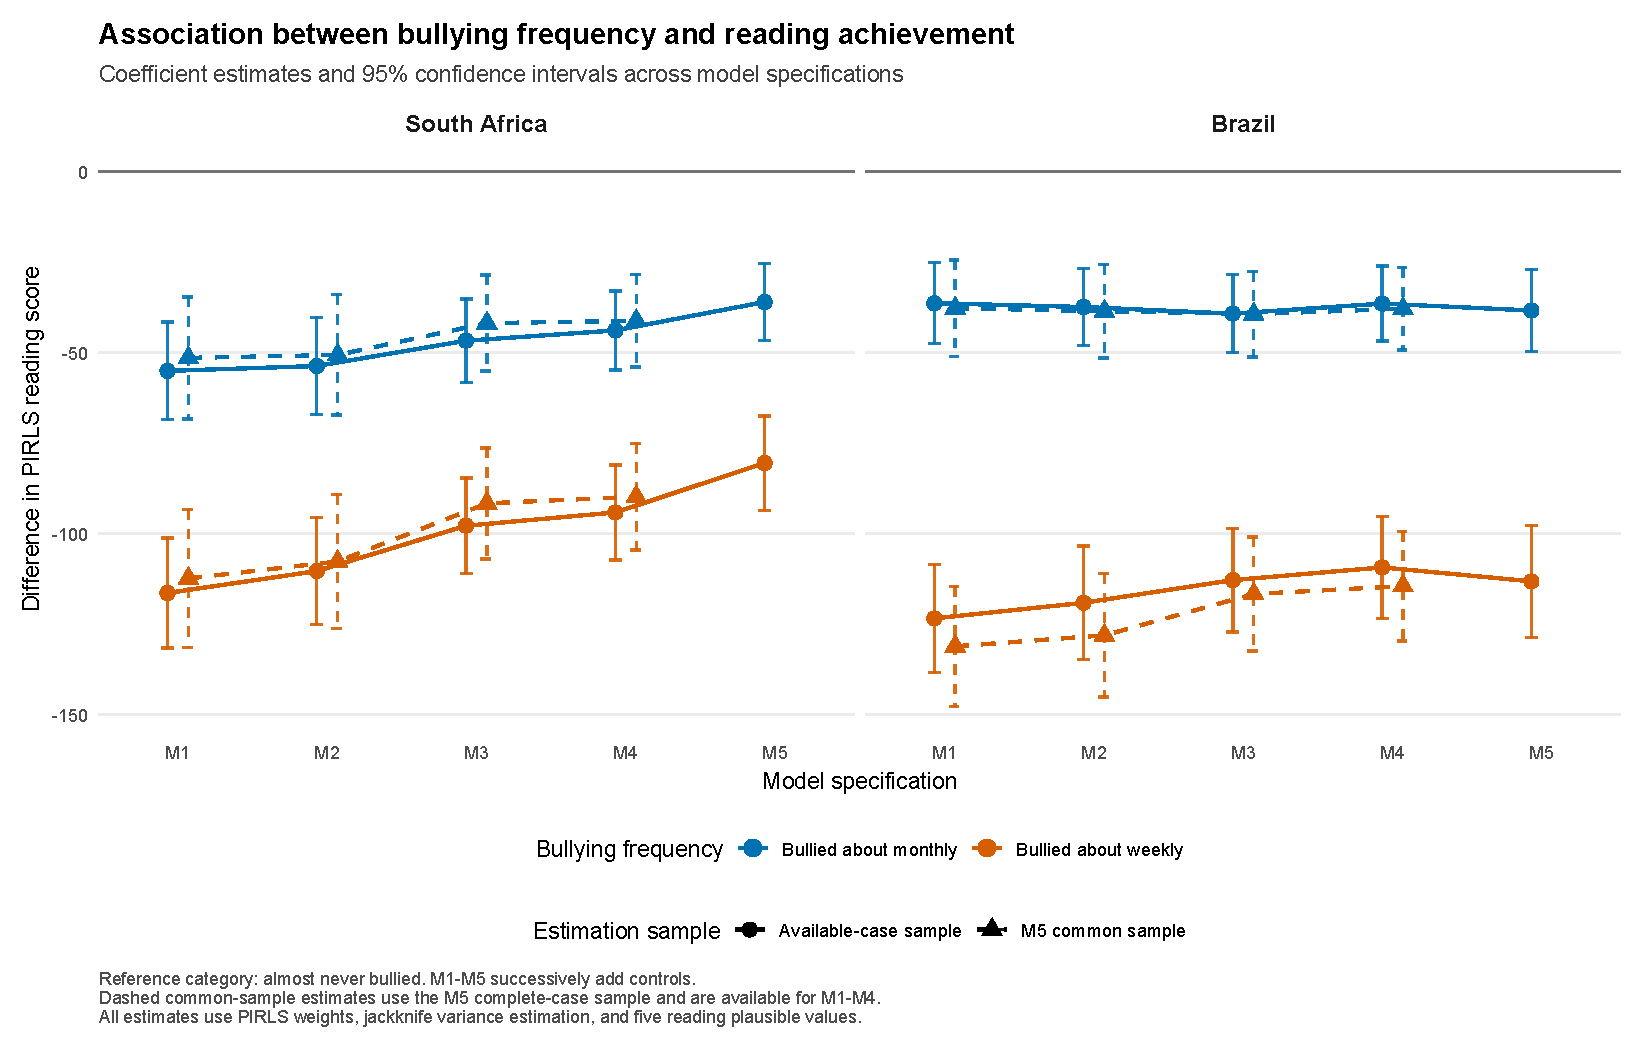
\includegraphics[width=\textwidth]{../../output/regressions/figures/bullying_coefficients_across_models.pdf}
\caption{Estimated association between bullying frequency and reading achievement across model specifications}
\label{fig:bullying-coefficients}
\end{figure}
\FloatBarrier

Re-estimating M1–M4 on the common M5 sample produced a similar pattern of coefficients, suggesting that the changes across models were not primarily attributable to sample composition (Appendix Table~\ref{tab:bullying-common-sample}). The continuous-scale specification also produced results consistent with the main analysis (Appendix Table~\ref{tab:bullying-robustness}).

Table~\ref{tab:bullying-interactions} presents the interactions between bullying and gender (I1) and between bullying and home SES (I2). The gender interactions are not statistically significant in either South Africa or Brazil. There is therefore no evidence that the association between bullying and reading achievement differs between boys and girls.

The SES interaction produces a different pattern. In South Africa, each one-unit increase in home SES makes the estimated monthly bullying penalty 13.2 points more negative and the weekly penalty 20.3 points more negative. In Brazil, the corresponding interaction coefficients are positive: 3.2 points for monthly bullying and 9.0 points for weekly bullying. The monthly interaction is not statistically significant, whereas the weekly interaction is significant at the 5\% level. Thus, there is evidence that higher SES intensifies the bullying penalty in South Africa, while the Brazilian estimates provide limited evidence that higher SES moderates the weekly bullying penalty.

\begin{table}[!htbp]
\centering
\caption{Heterogeneity in the association between bullying and reading achievement}
\label{tab:bullying-interactions}
\scriptsize
\setlength{\tabcolsep}{2.2pt}
\resizebox{\textwidth}{!}{%
\begin{tabular}{lcccc}
\toprule
 & \multicolumn{2}{c}{South Africa} & \multicolumn{2}{c}{Brazil} \\
\cmidrule(lr){2-3}\cmidrule(lr){4-5}
 & I1 & I2 & I1 & I2 \\
\midrule
Bullied about monthly & \shortstack{-46.5***\\(7.0)} & \shortstack{-42.2***\\(5.7)} & \shortstack{-34.1***\\(8.8)} & \shortstack{-39.8***\\(5.6)} \\
Bullied about weekly & \shortstack{-95.3***\\(7.8)} & \shortstack{-95.5***\\(6.4)} & \shortstack{-120.4***\\(10.6)} & \shortstack{-110.9***\\(6.9)} \\
Boy & \shortstack{-41.2***\\(6.7)} & \shortstack{-42.9***\\(3.4)} & \shortstack{-4.1\\(4.9)} & \shortstack{-5.6\\(4.7)} \\
Age (years) & \shortstack{-7.6**\\(3.4)} & \shortstack{-8.0**\\(3.4)} & \shortstack{-12.9***\\(4.4)} & \shortstack{-13.5***\\(4.3)} \\
Home SES (ASBHSES scale points) & \shortstack{25.7***\\(2.3)} &  & \shortstack{26.2***\\(2.1)} &  \\
Bullied about monthly × Boy & \shortstack{-0.7\\(9.4)} &  & \shortstack{-10.5\\(11.1)} &  \\
Bullied about weekly × Boy & \shortstack{-5.1\\(7.4)} &  & \shortstack{9.9\\(12.7)} &  \\
Home SES (centred scale points) &  & \shortstack{37.5***\\(2.8)} &  & \shortstack{24.1***\\(2.0)} \\
Bullied about monthly × Home SES (centred scale points) &  & \shortstack{-13.2***\\(2.8)} &  & \shortstack{3.2\\(3.0)} \\
Bullied about weekly × Home SES (centred scale points) &  & \shortstack{-20.3***\\(2.8)} &  & \shortstack{9.0**\\(4.5)} \\
Other gender category &  &  &  & \shortstack{-86.7**\\(35.2)} \\
\midrule
Learners & 9,167 & 9,167 & 4,076 & 4,110 \\
$R^{2}$ & 0.278 & 0.289 & 0.314 & 0.319 \\
\bottomrule
\end{tabular}%
}
\parbox{0.98\textwidth}{\footnotesize \textit{Notes:} Entries are coefficients with jackknife standard errors in parentheses. I1 interacts bullying with gender and excludes Brazil's 41 learners in the Other gender category. I2 interacts bullying with continuous ASBHSES centred at the design-weighted country mean; one unit is one PIRLS ASBHSES scale point. The reference bullying category is almost never and the gender reference is girls. Significance: *** p\textless{}0.01, ** p\textless{}0.05, * p\textless{}0.10.}
\end{table}

\FloatBarrier


\section{Conclusion}


\clearpage
\appendix
\section{Sensitivity and robustness analyses}

\begin{table}[!htbp]
\centering
\caption{Common-sample sensitivity analysis}
\label{tab:bullying-common-sample}
\scriptsize
\setlength{\tabcolsep}{2.2pt}
\resizebox{\textwidth}{!}{%
\begin{tabular}{lcccccccc}
\toprule
 & \multicolumn{4}{c}{South Africa} & \multicolumn{4}{c}{Brazil} \\
\cmidrule(lr){2-5}\cmidrule(lr){6-9}
 & M1 & M2 & M3 & M4 & M1 & M2 & M3 & M4 \\
\midrule
Bullied about monthly & \shortstack{-51.5***\\(8.6)} & \shortstack{-50.7***\\(8.5)} & \shortstack{-41.9***\\(6.8)} & \shortstack{-41.2***\\(6.5)} & \shortstack{-37.8***\\(6.8)} & \shortstack{-38.6***\\(6.6)} & \shortstack{-39.4***\\(6.0)} & \shortstack{-37.9***\\(5.8)} \\
Bullied about weekly & \shortstack{-112.5***\\(9.7)} & \shortstack{-107.8***\\(9.5)} & \shortstack{-91.7***\\(7.8)} & \shortstack{-89.9***\\(7.5)} & \shortstack{-131.2***\\(8.5)} & \shortstack{-128.2***\\(8.7)} & \shortstack{-116.8***\\(8.0)} & \shortstack{-114.6***\\(7.7)} \\
Boy &  & \shortstack{-45.5***\\(4.3)} & \shortstack{-43.1***\\(4.1)} & \shortstack{-41.4***\\(4.1)} &  & \shortstack{-5.9\\(5.7)} & \shortstack{-4.5\\(4.9)} & \shortstack{-3.2\\(4.8)} \\
Age (years) &  & \shortstack{-5.9\\(3.9)} & \shortstack{-5.5\\(3.7)} & \shortstack{-6.6*\\(3.6)} &  & \shortstack{-24.7***\\(5.2)} & \shortstack{-13.8***\\(4.7)} & \shortstack{-13.5***\\(4.7)} \\
Home SES (ASBHSES scale points) &  &  & \shortstack{26.5***\\(2.6)} & \shortstack{25.4***\\(2.6)} &  &  & \shortstack{25.7***\\(2.2)} & \shortstack{25.7***\\(2.2)} \\
Home language: almost always test language &  &  &  & \shortstack{9.1\\(9.2)} &  &  &  & \shortstack{-20.2*\\(11.4)} \\
Home language: sometimes test language &  &  &  & \shortstack{46.8***\\(7.9)} &  &  &  & \shortstack{12.4\\(9.6)} \\
Home language: never test language &  &  &  & \shortstack{-24.6**\\(10.1)} &  &  &  & \shortstack{-87.7***\\(19.4)} \\
Other gender category &  &  &  &  &  & \shortstack{-72.9***\\(24.3)} & \shortstack{-53.4**\\(24.0)} & \shortstack{-50.2**\\(24.4)} \\
\midrule
Learners & 7,177 & 7,177 & 7,177 & 7,177 & 3,563 & 3,563 & 3,563 & 3,563 \\
$R^{2}$ & 0.123 & 0.156 & 0.275 & 0.296 & 0.156 & 0.177 & 0.317 & 0.328 \\
\bottomrule
\end{tabular}%
}
\parbox{0.98\textwidth}{\footnotesize \textit{Notes:} Entries are coefficients with jackknife standard errors in parentheses. All models use the M5 complete-case sample. Significance: *** p\textless{}0.01, ** p\textless{}0.05, * p\textless{}0.10.}
\end{table}

\FloatBarrier

\begin{table}[!htbp]
\centering
\caption{Continuous-bullying robustness model}
\label{tab:bullying-robustness}
\scriptsize
\setlength{\tabcolsep}{2.2pt}
\resizebox{\textwidth}{!}{%
\begin{tabular}{lcc}
\toprule
 & \multicolumn{1}{c}{South Africa} & \multicolumn{1}{c}{Brazil} \\
\cmidrule(lr){2-2}\cmidrule(lr){3-3}
 & R1 & R1 \\
\midrule
Bullying scale (higher = less bullying) & \shortstack{18.7***\\(1.3)} & \shortstack{16.8***\\(1.2)} \\
Boy & \shortstack{-43.7***\\(3.6)} & \shortstack{-5.0\\(4.8)} \\
Age (years) & \shortstack{-8.0**\\(3.4)} & \shortstack{-13.7***\\(4.9)} \\
Home SES (ASBHSES scale points) & \shortstack{26.1***\\(2.3)} & \shortstack{27.4***\\(2.1)} \\
Other gender category &  & \shortstack{-97.7**\\(36.8)} \\
\midrule
Learners & 9,167 & 4,110 \\
$R^{2}$ & 0.270 & 0.293 \\
\bottomrule
\end{tabular}%
}
\parbox{0.98\textwidth}{\footnotesize \textit{Notes:} Entries are coefficients with jackknife standard errors in parentheses. Higher ASBGSB values indicate less bullying. Significance: *** p\textless{}0.01, ** p\textless{}0.05, * p\textless{}0.10.}
\end{table}

\FloatBarrier

\bibliographystyle{apalike}
\bibliography{references}

\end{document}
